\documentclass[a4paper]{IEEEtran}
\usepackage[utf8]{inputenc}
\usepackage{color}
\usepackage{graphicx}
\usepackage{mwe}
\usepackage{amsmath}
\usepackage{booktabs}
\usepackage{multicol}

\title{Malware Analysis Report\\\Large{``Sample2.exe''}}
\author{
    \begin{tabular}{lr}
        Contro Filippo &VR437055\\
        Martini Michele &VR437056
    \end{tabular}
}

\begin{document}
	\maketitle
	\section{Executive summary}
	The malware ``Sample2.exe'' shows itself as a calculator app, with the appropriate icon and the expected behavior. Once it is opened by the user there is a simple GUI to perform basic arithmetic operations. Under the hood, however, the malware deactivates the Windows security center, makes many POST request to various internet sites and infects many other files in different locations, from the local folder to the system application's executable.
	
	The whole analysis process has been done on the provided virtual machine, which runs Windows 7 as operating system and contains a bunch of tools to make both static and dynamic analysis. The reverse engineering instead has been done on local machines.
	
	\section{Static analysis}
	We began the static analysis using \emph{PEStudio}\footnote{https://www.winitor.com/}, a tool which performs malware initial assessment, studying headers, sections and many other features of the executable, which is never executed.
	This first analysis gave us many indicators of probable malicious behavior.
	First of all, in the main view we noticed an \emph{entropy} value greater than 7, therefore it's likely that either the file has been packed or some sections has been obfuscated. Entropy is a measure of the order of the application, and it is calculated with statistical operations on the bytes; As explained in this article\footnote{http://n10info.blogspot.com/2014/06/entropy-and-distinctive-signs-of-packed.html} 
	
	``When a section of code of a file is compressed, the total entropy will increase while counting, i.e. , it will get closer to the standard sum of all bits - this will mean higher efficiency of information storage, i.e., possible compression of section of code.

	\begin{figure}[htp]
		\frame{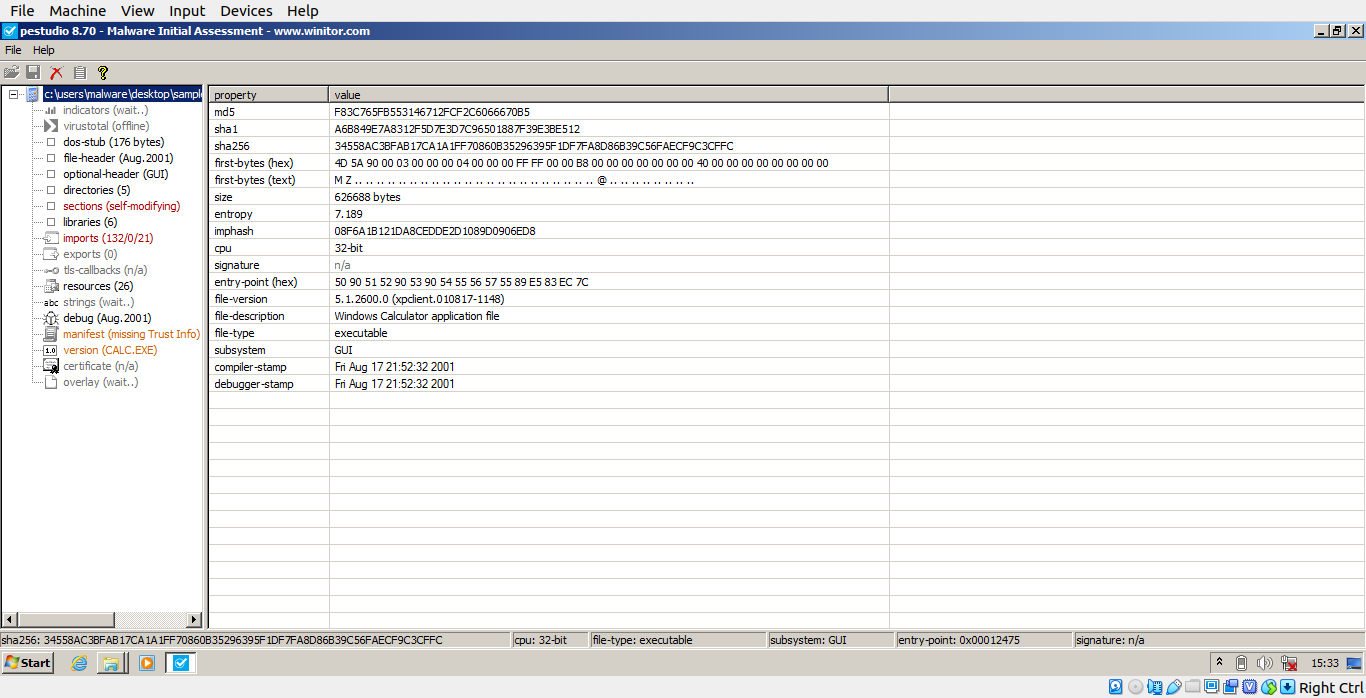
\includegraphics[width=0.5\textwidth]{img/PEStudio-main.png}}
	\end{figure}

	The maximum value for entropy in PEStudio is 8, so this high value is a clear evidence of packing and/or obfuscation.
	
	The executable lacks of any certificate, while the information dealing with the version disguise it as a ``Windows calculator application file'', with the legal copyright by Microsoft, but there is not a date. The header instead has a compilation time-stamp dating August 2001.

	\subsection{Sections}

	\noindent The malware's code is made up of four sections:
	\begin{itemize}
		\item \textbf{.text}: the code in clear;
		\item \textbf{.data}: contains global variables;
		\item \textbf{.rsrc}: contains various resources, like images or icons;
		\item \textbf{.vmp0}: main section of the code, obfuscated to make reverse-engineering more difficult.
	\end{itemize}

	\begin{figure}[bp]
		\frame{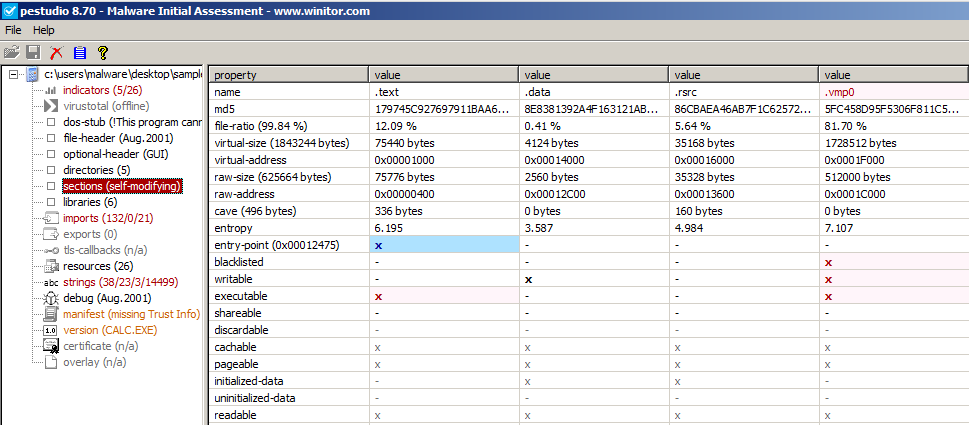
\includegraphics[width=0.5\textwidth]{img/PEStudio-sections.png}}
	\end{figure}

	The last section is the largest with a file-ratio of 81.70\%; it has an entropy greater than 7  and PEStudio marks it as blacklisted. Moreover it is both writable and executable, which is often a malicious evidence, as it indicates self modifying code.
	
	After a little search on the internet we discovered that the name ``vmp'' refers to an obfuscation program called \emph{VMProtect}\footnote{https://vmpsoft.com/}. This program cypher the code exectuting it in a virtual CPU that is different from $x86$. This code obfuscator makes the reverse engineering extremely difficult.
	
	Nevertheless, the presence of these sections allows us to suppose that the code has not been packed and its high entropy is due only to the ``vmp0'' section, which is obfuscated. In order to validate this theory, we used \emph{PEiD}, a software whose goal is to detect any possible packing. This tool provides three levels of analysis varying in depth. Every level, however, gave us the same result: ``nothing found'', meaning that PEiD could not detect any packing mechanism.

	\begin{figure}[htp]
		\frame{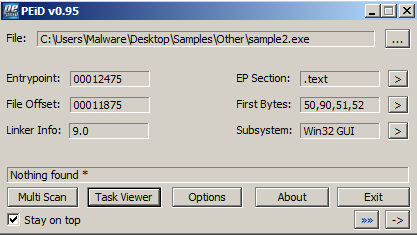
\includegraphics[width=0.5\textwidth]{img/PEiD.png}}
	\end{figure}

	\subsection{Imports}
	
	The executable imports 6 libraries in total, and in particular PEStudio marks as blacklisted 21 functions belonging to \emph{Kernel32.dll} and \emph{user32.dll}. The most interesting are:

	\begin{itemize}
		\item \textbf{getModuleHandleA}, to call external files, such as \emph{dll} or \emph{exe};
		\item \textbf{loadLibraryA}, similar to that one above;
		\item \textbf{getProcAddress}, to get the address of a procedure inside a library;
		\item \textbf{getStartupInfoA}, to get information about startup;
		\item \textbf{getCommandLineW}, to let the program execute code on the command line;
	\end{itemize}
	
	Moreover there are also imports of functions dealing with \emph{Threads}, \emph{Clipboard} and \emph{Windows}.
	This suggests a suspicious behavior, due to the possibility of the program to access to all the libraries of the installed operating system.
	In the dynamic analysis we will see what actions are actually performed.
	The figure below contains all the blacklisted imports detected by PEStudio.
	
	\begin{figure}[htp]
		\frame{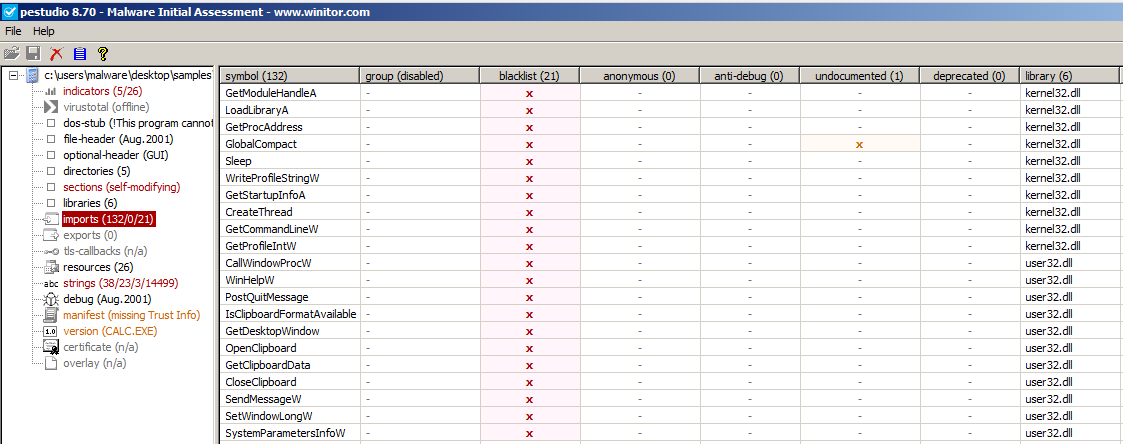
\includegraphics[width=0.5\textwidth]{img/PEStudio-imports.png}}
	\end{figure}
	
	%TODO Indicators and import analysis
	
	\subsection{Strings}
	Regarding strings we notice that those in .text, .data and .rsrc sections are in clear; furthermore many of them are function calls or values used to modify system registers.
	Followin them there are thousands of obfuscated strings, seemingly meaningless, which belong to the ``.vpm0'' section. This is another clue of code obfuscation.	
	
	
	\section{Dynamic analysis}
	
	The dynamic analysis consists of the execution of the malware in a controlled and isolated system to observe the behavior and the malicious actions performed.
	
	To accomplish this task we used \emph{VirtualBox}, a virtualization program that let us run a Windows 7 machine. VirtualBox handles the snapshots too, so that after every test the machine was restored to its initial state. The machine was also isolated from internet in order to avoid leaks.
	
	The machine was equipped with various tools to monitor the execution of the malware. The main ones were:
	\begin{itemize}
		\item \textbf{regshot}, to detect files and registers alterations between a time lapse;
		\item \textbf{procmon}, to log system functions called by the malware;
		\item \textbf{fakenet}, to track internet traffic in a simulated network.
	\end{itemize}
	These programs were executed with administrator permission in order to detect access to restricted locations.
	
	The tools can cooperate but they need to be executed is a certain schedule, in order to avoid conflicts among them. The analysis proceeded following these phases:
	\begin{enumerate}
		\item launch Fakenet;
		\item launch and setup Procmon;
		\item launch Regshot, setup path and run of its first shot;
		\item start Procmon analysis and launch of the malware;
		\item interaction with calculator by the GUI;
		\item stop Procmon tracking
		\item second Regshot shot;
		\item stop Fakenet;
	\end{enumerate}
	
	The first tests did not last too long: the GUI remained opened for just a few seconds. These tests did not give us evidence of malicious behavior, probably beacuse of the poor performance of the host machine.

	Then we ran other test leaving the malware run for a couple of minutes, leaving all the time needed to permorm bad actions. Then we collect the logs and analyzed them one by one.

	The first evidence of malicious behavior has been observed without any tools. After 20-30 seconds from the program execution the operating system prompted us a message about the \emph{Windows security center}; it was disabled and, from the control panel, it could not be re-activated. This is a seriuos threat to the security of the machine, leaving it opened to many other infections.

	\begin{figure}[htp]
		\frame{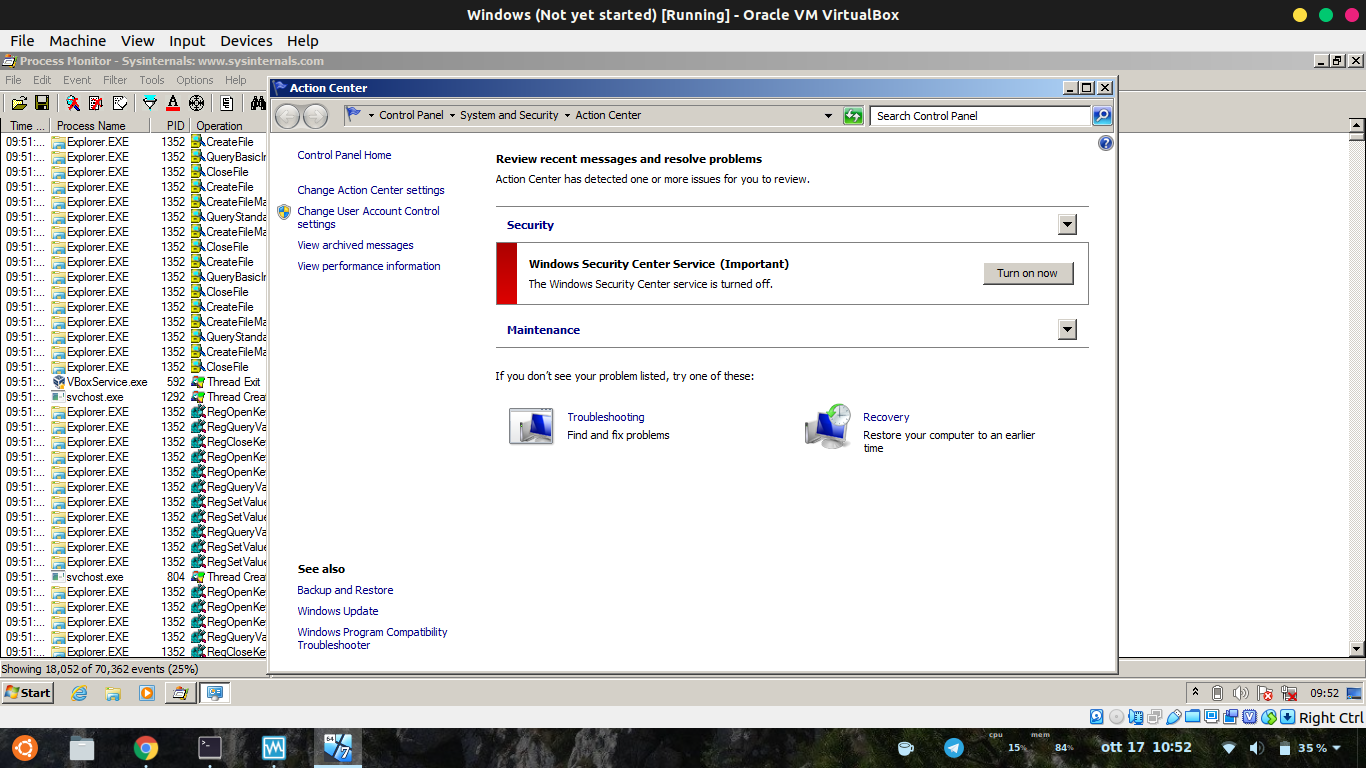
\includegraphics[width=0.5\textwidth]{img/securityCenter.png}}
	\end{figure}

	\subsection{Fakenet}

	FakeNet is a dynamic network analysis tool for malware analysts and penetration testers. It simulates a network logging the traffic generated by the machine. Every request is a file containing:

	\begin{itemize}
		\item Request type
		\item Destination URL
		\item Protocol
		\item User agent
	\end{itemize}

	The user agent field contains various informations about the local machine, such as architecture, operating system, product and so on. This string is
	\begin{quote}
		\texttt{User-Agent: Mozilla/4.0\\ (compatible; MSIE 28;\dots}
	\end{quote}
	

	The registered requests are over 900, whereas the destintions are 300, mainly russian sites. Unluckily the body is empty, and we cannot know the expected result due to the precsence of fakenet, which builds a fake http page as response to every request.

	\subsection{Procmon}

	\subsection{RegShot}
	
	
	\section{Reverse Engineering}
\end{document}